\chapter{RD53A}

Il progetto di RD53A è stato approvato nell'autunno del 2015, dopo la revisione da parte delle collaborazioni ATLAS, CMS e RD53A. Nel 2016 è iniziata la progettazione del chip, con RD53A si vuole dimostrare la possibilità di utilizzare tecnologia CMOS  in 65 nm per l'aggiornamento in vista della fase ad alta luminosità di ATLAS e CMS, e quindi la tolleranza al danneggiamneto da radiazioni, soglie di lavoro basse e stabili nel tempo, capacità di gestire un alto flusso di particelle incidenti e l'utilizzo di trigger veloci. 
RD53A non deve essere inteso come il prodotto finale, infatti possiede molte modifiche di desing utili solo in una prima fase di test, ad esempio al suo interno sono presenti tre diversi front-end (FE), già questo causa una non uniformità del chip. 
Questo chip è la base di partenza per arrivare al progetto finale, in cui sarà scelto uno dei front end e sarà utilizzato uniformemente su tutta la matrice di pixel. In RD53a la matrice di pixel ha 400 colonne e 192 righe, nel progetto finale si avrà un aumento del numero di pixel, infatti il sistema di alimentazione e di contropolarizzazione dei pixel è progettato per un numero di righe massimo pari a 384, figura \ref{RD53ALayout}.
\begin{figure}
\centering
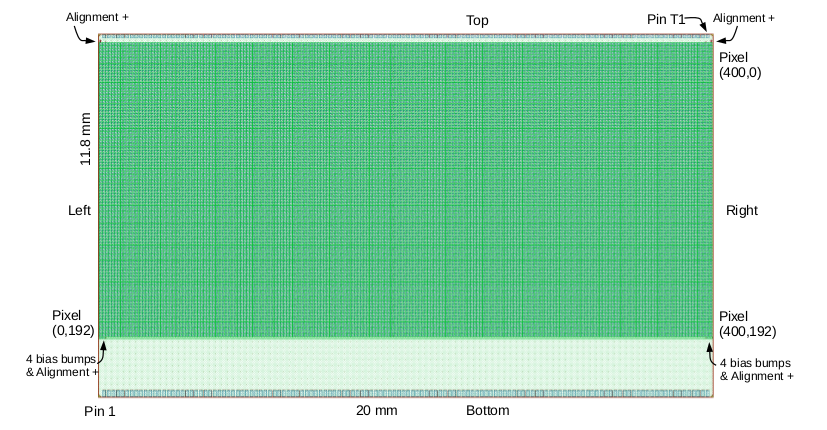
\includegraphics[scale=.4]{Immagini/RD53ALayout}
\caption{RD53A layout. Il chip è largo 20mm per 400 pixel e l'altezza è 11.8 mmm per 192 pixel.}
\label{RD53ALayout}
\end{figure}

L'area del chip che sarà bondata al sensore è posta nella parte alta ed è organizzata secondo una matrice di 192 x 400 pixel di area 50 $\mu$m x 50 $\mu$m, sopra a questa è presente una fila di pad utilizzate per debug, questa sarà eliminata nella versione finale. La parte di circuito necessaria per configurare monitorare e leggere il chip è posta nella parte bassa, sotto cui è posta una fila di pad per i wire-bond. 
La matrice di pixel è organizzata in \textit{cores} di 8 x 8 pixel, all'interno i 64 front end sono disposti in gruppi di 4, chiamati isole analogiche. 
Queste isole sono circondate da un "mare" digitale, il circuito introno ad ogni isola è differente. 
Nelle parti più esterne del chip tutti i blocchi analogici sono raggruppati in macro blocchi chiamati Analog Chip Bottom (ACB). Il blocco ACB è circondato dal blocco Digital Chip Bottom (DCB) che implementa la logica digitale per Input, Output e configurazione.

\section{SLDO}
In RD53A la parte di SLDO differisceda quella presente sulla PCB di test, in particolare la tensione di offset è generata con un circuito diverso, vedi figura \ref{SLDO_RD53A}. Infatti, è possibile applicare al terminale $I_{ofs}$ una resistenza che con la sua caduta di tensione determina il valore di $V_{ofs}$. 
Questa resistenza va saldata sulla Single Chip Card nell'apposito slot. Il valore di $I_{ofs}$ è 2 $\mu$A, quindi:
\begin{equation}
V_{ofs} = 2 \mu m \cdot R_{iofs}
\end{equation}
Questa tensione viene raddopiata tramite l'azione dell'anello di reazione di A5, prima di essere mandata ad A4.
Riepilogando il comportamento della tensione in ingresso sarà:
\begin{equation}
V_{in}= 2 \cdot V_{ofs} + \dfrac{R3}{1000} \cdot I_{in}
\end{equation}
Nelle misure che sono presentate nelle sezioni sucessive ogni volta che si parlerà di R3 e $V_{ofs}$ interni si farà riferimento ai seguenti valori:

\begin{center}
\begin{tabular}{lc}
\hline
$\mathrm{R3}$ & 620 $\Omega$ \\
$\mathrm{R_{iofs}}$ & 250 k$\Omega$\\ 
\hline
\end{tabular}
\end{center}

\begin{figure}
\centering
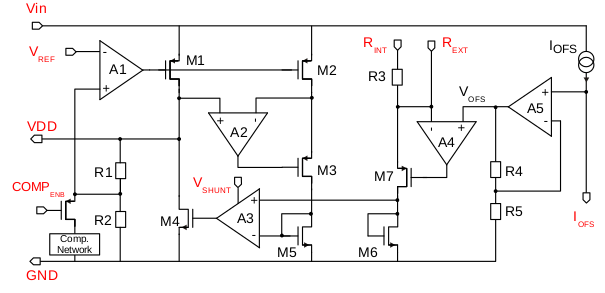
\includegraphics[scale=.6]{Immagini/SLDO_RD53A}
\caption{.}
\label{SLDO_RD53A}
\end{figure}

Per quanto riguarda le tensioni di riferimento, come $V_{ref}$, queste vengono generate all'interno del chip da un circuito dedicato in cui vengono utilizzati bandgap. Il valore di uscita dei bandgap è configurabile, di default ha un valore 16 

\section{Single Chip Card}


\begin{figure}
\centering
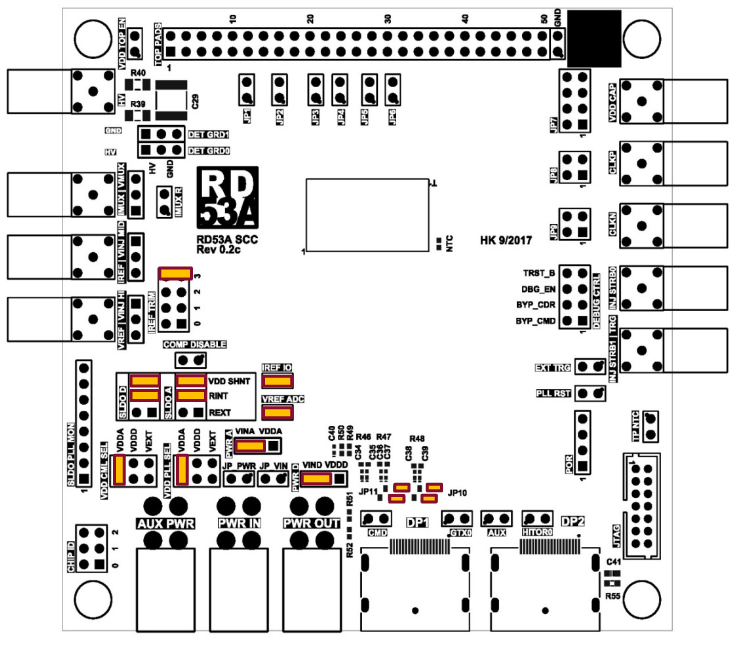
\includegraphics[scale=.3]{Immagini/SLDOmode}
\caption{Configurazione di default .}
\label{SLDOmode}
\end{figure}
\begin{figure}
\centering
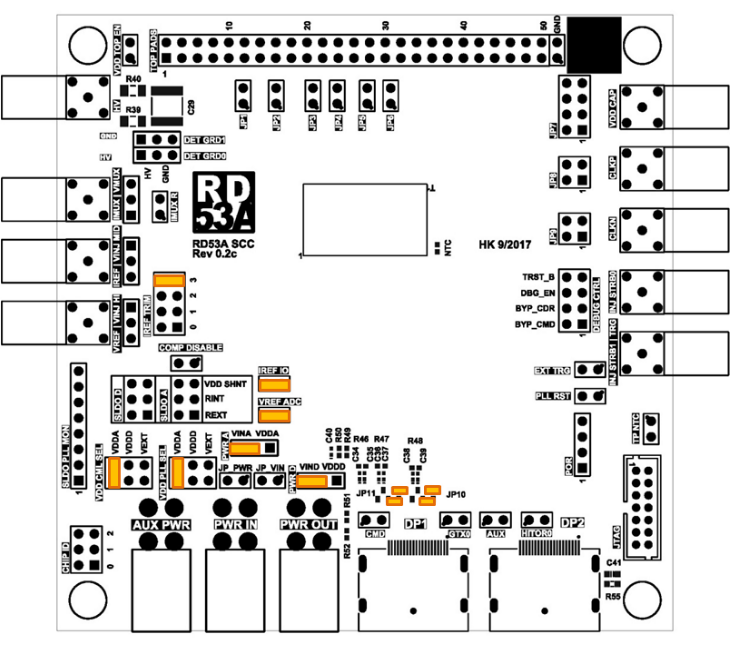
\includegraphics[scale=.3]{Immagini/LDOmodeDefault}
\caption{Configurazione di default .}
\label{LDOmodeDefault}
\end{figure}
\begin{figure}
\centering
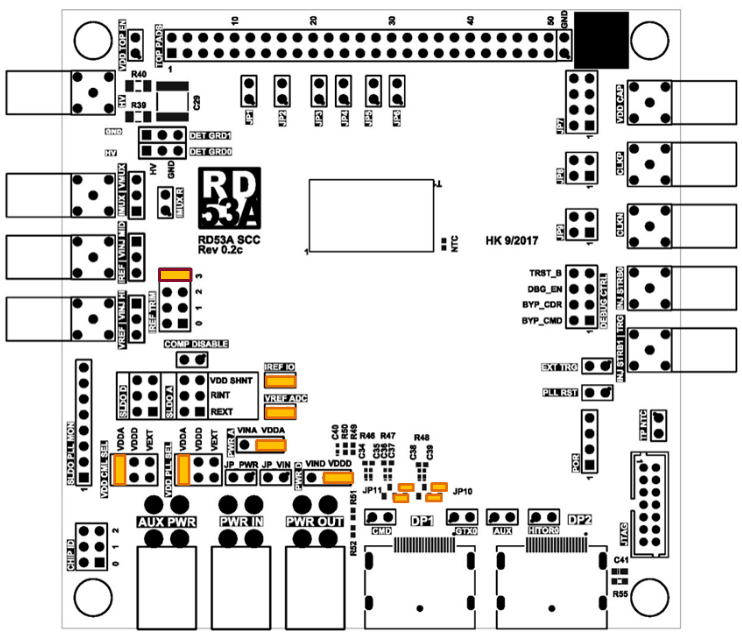
\includegraphics[scale=.3]{Immagini/DirectPowering}
\caption{Configurazione di default .}
\label{DirectPowering}
\end{figure}

\section{Misure Statiche con chip}
Misure in configurazione SLDO
\begin{figure}
\centering
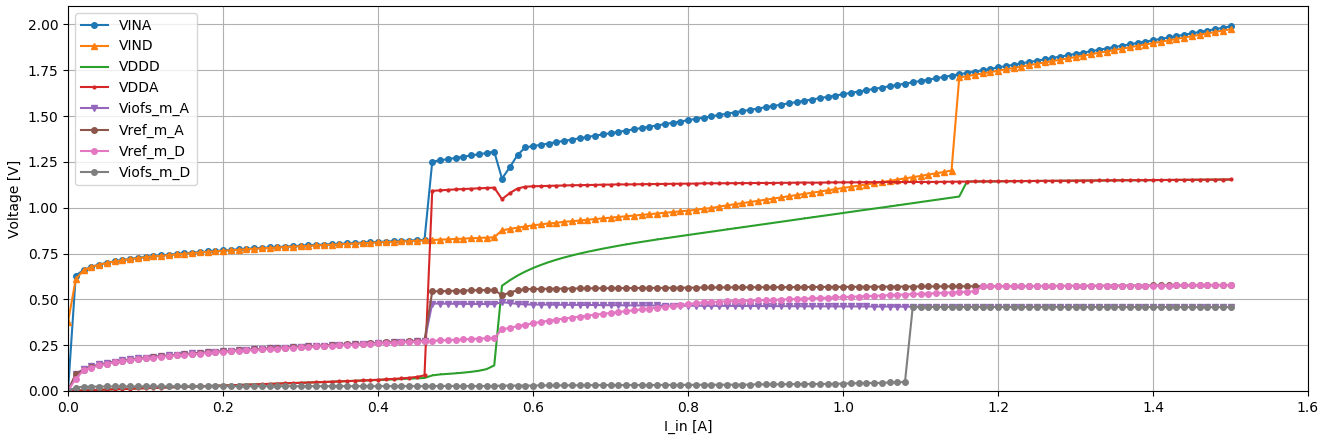
\includegraphics[scale=.3]{Immagini/IUI2}
\caption{.}
\label{IUI}
\end{figure}
causato da una distribuzione non uguale delle correnti nei due SLDO, quando si attiva la parte digitale ha un picco di assorbimento di corrente che causa un drop nella parte analogica. questo perchè benchè le alimentazioni siano separate all'interno del chip ci sono comunque zone di 'dialogo' tra regione analogica e digitale.



\begin{figure}
\centering
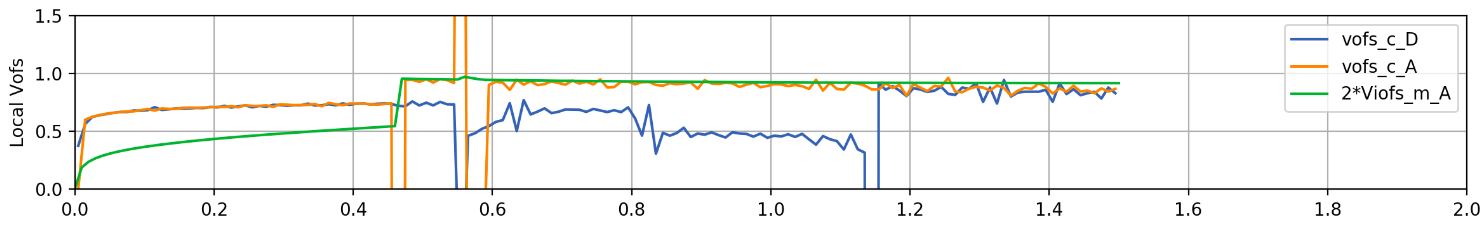
\includegraphics[scale=.27]{Immagini/IUISubPlotVofs}
\caption{.}
\label{IUISubPlotVofs}
\end{figure}

\begin{center}
\begin{tabular}{|l|c|c|}
\hline
&Digitale  &Analogica \\ \hline
$\mathrm{R_{eq}}$ & 0.753 $\Omega$& 0.724 $\Omega$ \\ \hline
$\mathrm{V_{ofs}}$ & 0.845 V & 0.900 V\\ \hline
\end{tabular}
\end{center}

\begin{figure}
\centering
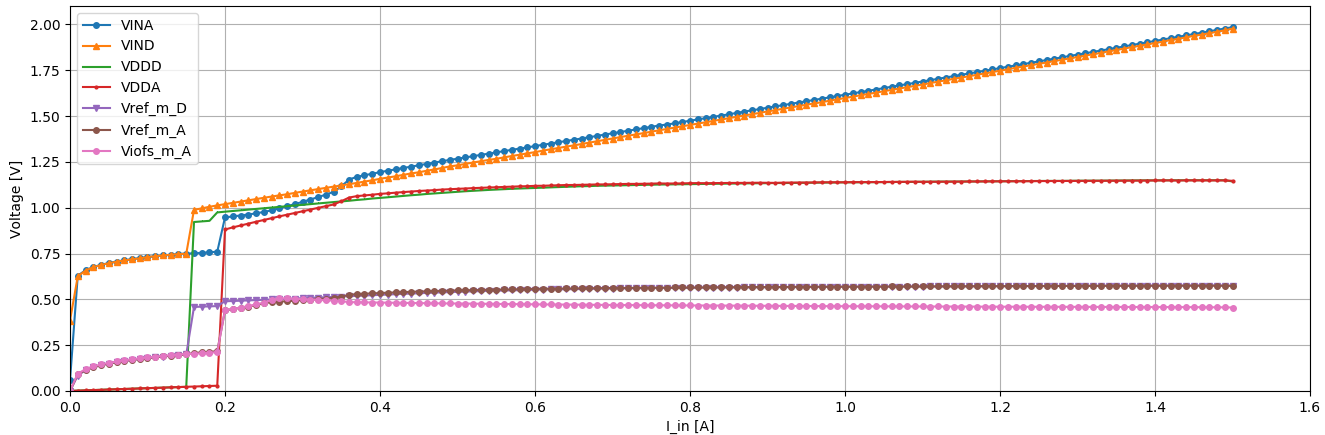
\includegraphics[scale=.3]{Immagini/IDI2}
\caption{.}
\label{IDI}
\end{figure}

\begin{figure}
\centering
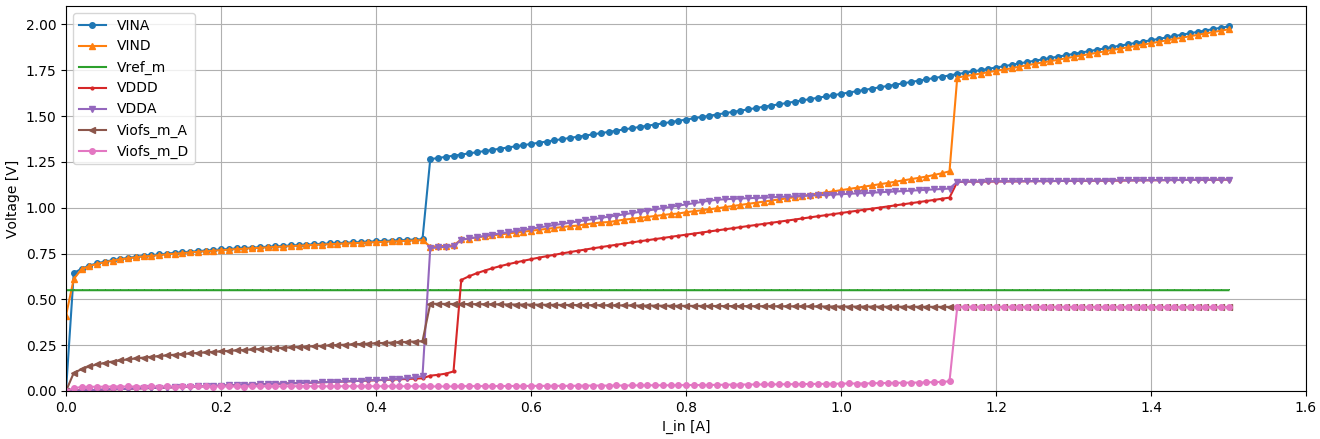
\includegraphics[scale=.3]{Immagini/IUEVref2}
\caption{.}
\label{IDEVref}
\end{figure}

\begin{figure}
\centering
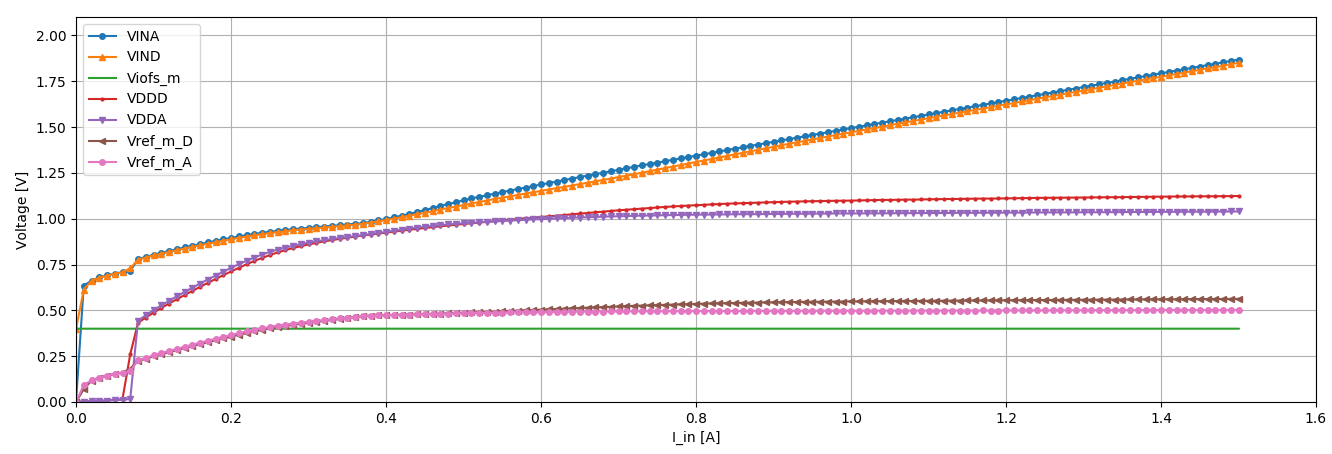
\includegraphics[scale=.3]{Immagini/IUEViofs2}
\caption{.}
\label{IDEViofs}
\end{figure}


\begin{figure}
\centering
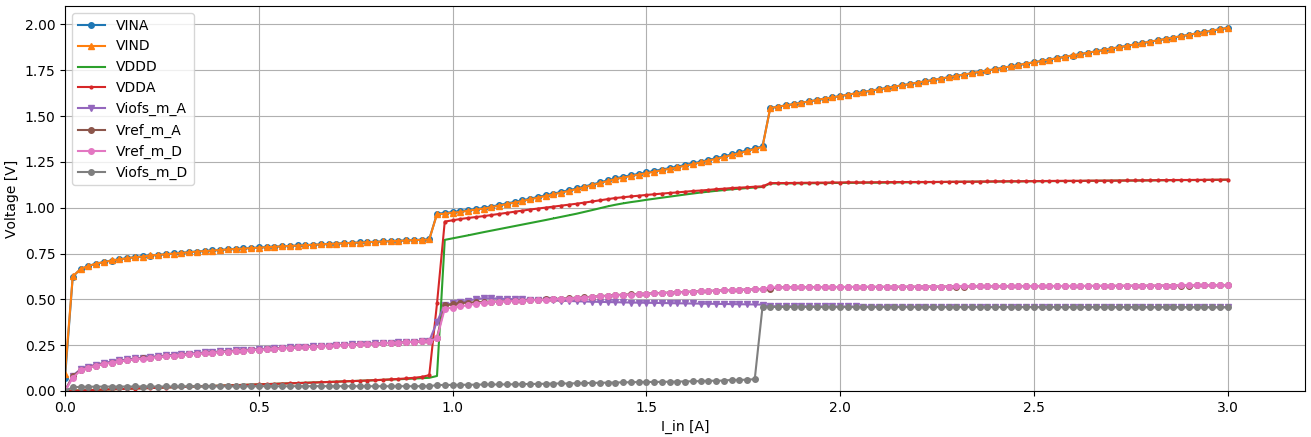
\includegraphics[scale=.3]{Immagini/PUI}
\caption{.}
\label{PUI}
\end{figure}





\afterpage{\clearpage}

\subsection{LDOvsSLDO}

\begin{figure}
\centering
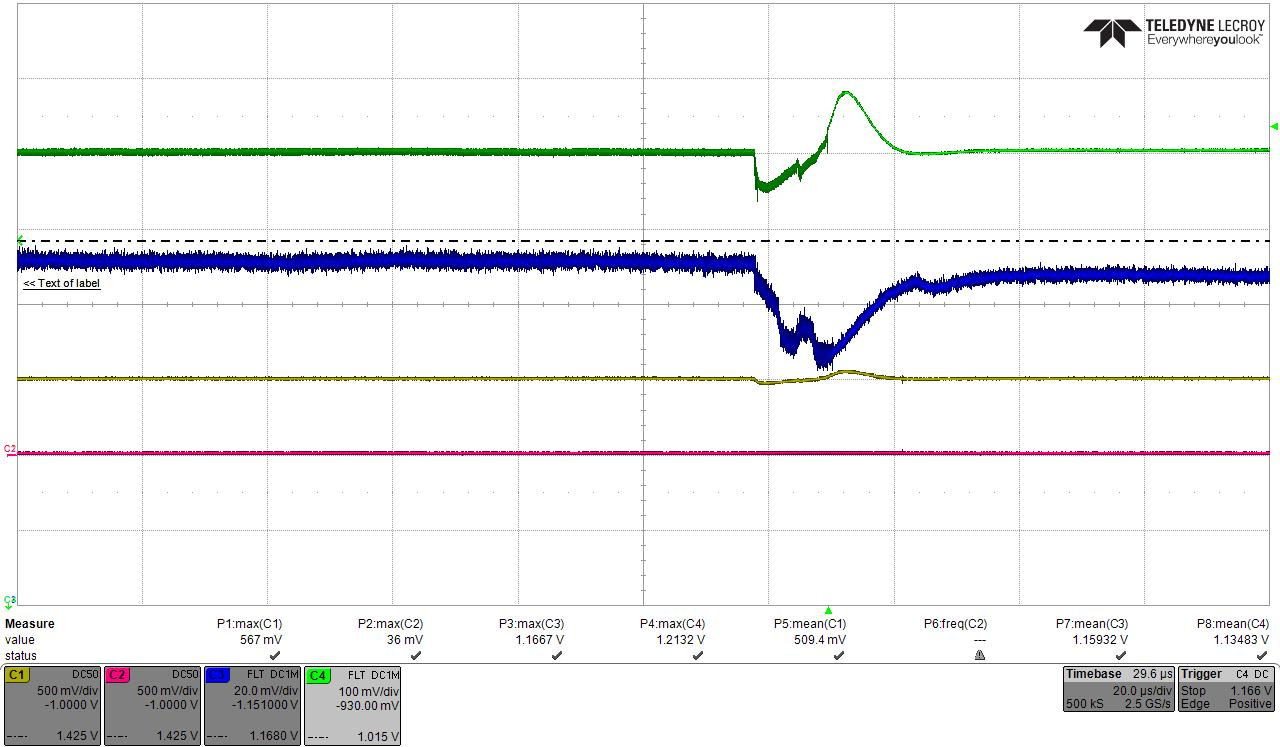
\includegraphics[scale=.3]{Immagini/alllin1}
\caption{.}
\label{alllin1}
\end{figure}

%\begin{figure}
%\centering
%\includegraphics[scale=.3]{Immagini/}
%\caption{.}
%\label{}
%\end{figure}

\section{Front End}
Come detto in precedenza RD53A non è il chip finale, ma un prototipo, al cui interno sono presenti tre differenti Front End per la parte anlogica. Si tratta di tre differenti progetti e sono indicati con i nomi: Sincrono, Lineare e Differenziale, vedi figura \ref{FrontEnd}. 
Questi tre circuiti sono stati progettati da tre differenti gruppi e tra di loro ci sono importanti differenze. Il FE Sincrono sfrutta un sistema di auto-zeroing della linea di base, campionando periodicamente la linea di base invecedi aggiutre la soglia pixel per pixel. 
Il Lineare implementa un amplificatore lineare all'ingesso del comparatore, il cui compito è confrontare il segnale con una certa soglia. 
Nel Differenziale è presente uno stadio di guadagno differenziale  all'ingresso del discriminatore e sbilanciando i due canali implementa la soglia..
Le caratteristiche comuni sono le piazzole per i bump-bond e il layout. Inoltre è comune anche la rete di polarizzazione ed il circuito per iniettare segnali di calibrazione, in modo da poter comparare direttamente le prestazioni. 
I tre FE condividono l'area del sensore e dato che la matrice è larga 400 pixel ed è suddivisa in core da 8 $\times$ 8 pixel, dunque non è possibile avere una egual area per i tre tipi di FE. Due avranno 17 core e uno solo ne avrà 16. I FE Lineare e Differenziale sono stati posti accanto in quanto hanno funzionalità simili e metterli vicino consente di avere un'area maggiore con una risposta il più uniforme possibile. 
\begin{figure}
\centering
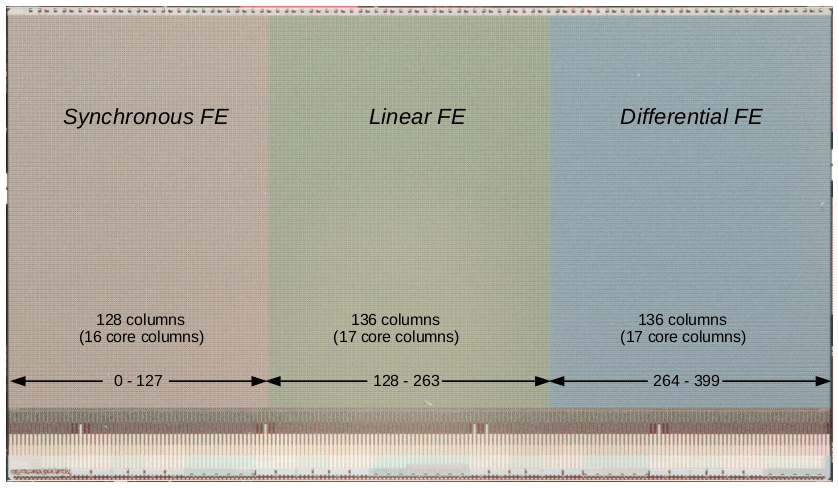
\includegraphics[scale=.3]{Immagini/FrontEnd}
\caption{.}
\label{FrontEnd}
\end{figure}

\begin{itemize}
\item \textbf{Torino}
\item \textbf{LBNL}
\item \textbf{Bonn}
\end{itemize}

\section{Sistemi di acquisizione dati}


\section{Setup}
LDO mode
%3.3 ESD Protection and Safe Wire Bonding
%
%%In the bottom pad frame the four power domains (VDDA, VDDD, VDD_CML, and VDD_PLL) are
%isolated by power-cut cells. Within a power domain group, the IO pad ESD devices are connected
%to the respective power rails. To allow an ESD path between power domains a common ESD
%bus connects to every power domain’s ground rail via sets of anti-parallel diodes. This ESD bus
%is also used to connect the global substrate of the chip (VSUB). !!!!!!Because the IO pads use ESD
%devices connecting to the power rails, care must be taken to not drive signals to the chip while it
%is not powered, as this would supply parasitic power. There are a few pads which have an over-
%voltage tolerant ESD protection without a current path to the power rail. These pads are used where
%the input voltage can exceed the VDDA/VDDD rail potentials (input- and bias pads of the shunt
%regulator blocks, for example). Where low capacitance is mandatory (CML driver output pads) a
%path to the VDDA/VDDD rails was also omitted.
%%The top test pads have an independent power domain (VDD_TOP/GND_TOP) which is not
%connected to the global ESD bus at the chip bottom. Within the top row the IO pads are protected
%but since there is no connection to the global ESD bus, ESD events between top and bottom pads
%should be avoided. The IO pads in the top pad frame are all over-voltage tolerant and therefore
%output signals are not clamped if the top row is not powered.
%The wire bonding sequence to avoid ESD problems is as follows: Start with the VSUB pads
%(14, 88 and 184) followed by all GND pads in any order. Finally bond the remaining pads in any
%order. The top row pads can be left floating, but if wire bonded then start with the GND pads (T2,
%T51 and T97) followed by the VDD pads (T1, T50 and T96) and then all other pads.
\section{Scansioni}


\section{Sviluppi}